\documentclass[aspectratio=169, 11pt]{beamer}

% ── Theme & Colors ──────────────────────────────────────────
\usetheme{Madrid}
\usecolortheme{default}

\definecolor{darkcharcoal}{HTML}{2C3E50}
\definecolor{accentblue}{HTML}{2980B9}
\definecolor{donegreen}{HTML}{27AE60}
\definecolor{pendinggray}{HTML}{BDC3C7}
\definecolor{lightbg}{HTML}{F8F9FA}
\definecolor{darktext}{HTML}{1A1A2E}

\setbeamercolor{structure}{fg=darkcharcoal}
\setbeamercolor{palette primary}{bg=darkcharcoal, fg=white}
\setbeamercolor{palette secondary}{bg=accentblue, fg=white}
\setbeamercolor{frametitle}{bg=darkcharcoal, fg=white}
\setbeamercolor{title}{fg=darkcharcoal}
\setbeamercolor{subtitle}{fg=accentblue}
\setbeamercolor{block title}{bg=darkcharcoal, fg=white}
\setbeamercolor{block body}{bg=lightbg, fg=darktext}
\setbeamercolor{item}{fg=accentblue}

\setbeamertemplate{navigation symbols}{}
\setbeamerfont{frametitle}{size=\large, series=\bfseries}
\setbeamerfont{title}{size=\Large, series=\bfseries}

% ── Packages ────────────────────────────────────────────────
\usepackage{tikz}
\usetikzlibrary{shapes.geometric, arrows.meta, positioning, fit, calc}
\usepackage{amsmath, amssymb}
\usepackage{booktabs}
\usepackage{graphicx}
\usepackage{hyperref}
\usepackage{xcolor}
\usepackage{array}

% ── TikZ Styles ─────────────────────────────────────────────
\tikzstyle{block} = [rectangle, rounded corners, minimum width=2.2cm, minimum height=0.8cm, text centered, draw=darkcharcoal, fill=lightbg, font=\small]
\tikzstyle{done} = [block, draw=donegreen, fill=donegreen!10, text=donegreen!80!black]
\tikzstyle{pending} = [block, draw=pendinggray, fill=pendinggray!15, text=pendinggray!60!black]
\tikzstyle{arrow} = [-{Stealth[length=2.5mm]}, thick, color=darkcharcoal!70]

% ── Meta ────────────────────────────────────────────────────
\title{Optimising Fed-Batch Feed-Flow Strategies}
\subtitle{UG Project Progress Report :  VIIth Semester}
\author{Yashashwi Singhania}
\date{September 2026}

% ═══════════════════════════════════════════════════════════
\begin{document}

\begin{frame}[plain]
  \vfill
  \begin{center}
    
\includegraphics[height=1.5cm]{iit_bhu_logo.png}\\[0.25cm]
    {\Large\bfseries\color{darkcharcoal} Indian Institute of Technology (BHU), Varanasi}\\[0.3cm]
    {\LARGE\bfseries\color{darkcharcoal} Optimising Fed-Batch}\\[0.15cm]
    {\LARGE\bfseries\color{darkcharcoal} Feed-Flow Strategies}\\[0.4cm]
    {\large\color{accentblue} UG Project 2: Semester Report}\\[0.4cm]
    \begin{tabular}{rl}
      \textbf{Student:} & Yashashwi Singhania (23014019) \\
      \textbf{Guide:} & Dr.\ Sharon Mano Pappu J. \\
      \textbf{Department:} & Biochemical Engineering \\
      \textbf{Lab:} & Bioprocess Development and Digitalization Laboratory \\
    \end{tabular}\\[0.25cm]
    {\small September 2026}
  \end{center}
  \vfill
\end{frame}

\begin{frame}{Project Roadmap}
  \begin{center}
  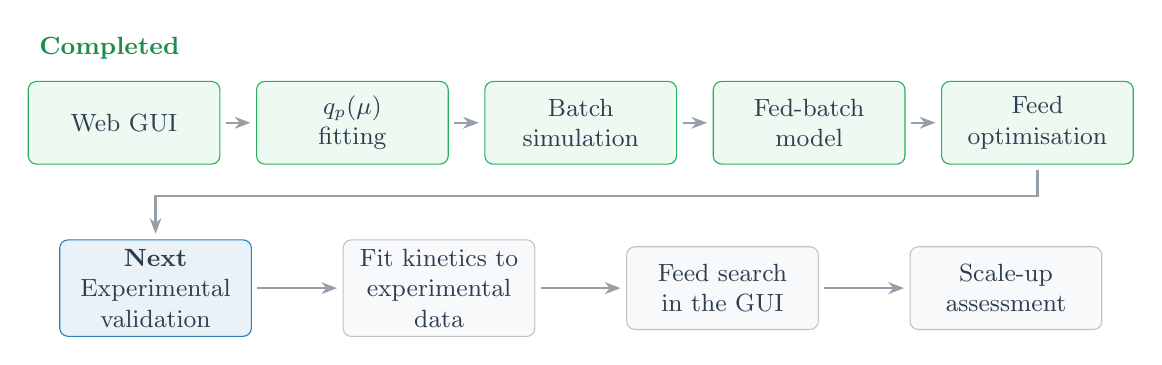
\begin{tikzpicture}[
    every node/.style={align=center},
    completed/.style={rectangle, rounded corners=3pt, draw=donegreen,
      fill=donegreen!8, text=darkcharcoal, text width=2.2cm,
      minimum height=1.05cm, font=\small},
    nextstep/.style={completed, draw=accentblue, fill=accentblue!10},
    planned/.style={completed, draw=pendinggray, fill=lightbg},
    arr/.style={-{Stealth[length=2mm]}, thick, color=darkcharcoal!50,
      shorten >=2pt, shorten <=2pt}]
    \node[font=\small\bfseries,text=donegreen!80!black,anchor=west] at (-1.2,0.95) {Completed};
    \node[completed] (a) at (0,0) {Web GUI};
    \node[completed] (b) at (2.9,0) {$q_p(\mu)$\\fitting};
    \node[completed] (c) at (5.8,0) {Batch\\simulation};
    \node[completed] (d) at (8.7,0) {Fed-batch\\model};
    \node[completed] (e) at (11.6,0) {Feed\\optimisation};
    \draw[arr] (a) -- (b); \draw[arr] (b) -- (c);
    \draw[arr] (c) -- (d); \draw[arr] (d) -- (e);
    \node[nextstep] (f) at (0.4,-2.1) {\textbf{Next}\\Experimental\\validation};
    \node[planned] (g) at (4,-2.1) {Fit kinetics to\\experimental data};
    \node[planned] (h) at (7.6,-2.1) {Feed search\\in the GUI};
    \node[planned] (i) at (11.2,-2.1) {Scale-up\\assessment};
    \draw[arr] (e.south) -- ++(0,-0.4) -| (f.north);
    \draw[arr] (f) -- (g); \draw[arr] (g) -- (h); \draw[arr] (h) -- (i);
  \end{tikzpicture}
  \end{center}
  \vspace{0.2cm}
  \begin{block}{Experimental validation}
    Compare predicted $X$, $S$ and $P$ with measured fed-batch data using the
    actual reactor, feed and pump conditions.
  \end{block}
\end{frame}

\begin{frame}{Growth Rate and Product Formation}
  \begin{block}{How feeding influences production}
    \centering
    $F(t)\ \longrightarrow\ S(t)\ \longrightarrow\ \mu(t)\ \longrightarrow\ q_p(\mu)$
  \end{block}
  \vspace{0.3cm}
  \begin{center}
    \renewcommand{\arraystretch}{1.5}
    \begin{tabular}{lll}
      \toprule
      \textbf{Shape} & \textbf{Relationship} & \textbf{Expected behaviour} \\
      \midrule
      Linear & $q_p=\alpha\mu+\beta$ & Higher growth raises $q_p$ \\
      Bell-shaped & Peak near $\mu_{\mathrm{opt}}$ & An intermediate growth rate helps \\
      Hyperbolic & $q_p=q_{p,\max}\mu/(K_q+\mu)$ & $q_p$ approaches a plateau \\
      \bottomrule
    \end{tabular}
  \end{center}
  \vspace{0.3cm}
  \textbf{Question:} which feed strategy gives the most total product under the same reactor constraints?
\end{frame}

\begin{frame}{Process Model}
  Every one of the 9 datasets runs in the \textbf{same generic reactor}, so only the
  fitted $q_p(\mu)$ relationship (and the organism's own $\mu_{max}/K_S/Y_{X/S}$) differs
  between runs.

  \vspace{0.2cm}
  \begin{columns}[T]
    \begin{column}{0.46\textwidth}
      \textbf{Batch phase} ($F=0$):\\
      {\small $X_0$=0.1 g/L, $S_0$=20 g/L, $V_0$=1 L, Monod kinetics until $S$ depletes
      to 0.5 g/L when the feed pump switches on.}
    \end{column}
    \begin{column}{0.5\textwidth}
      \textbf{Fed-batch phase} (fixed 40 h horizon):
      \begin{align*}
        \dot X &= \mu X - (F/V)X \\
        \dot S &= (F/V)(S_{in}-S) - (\mu/Y_{X/S})X \\
        \dot P &= q_p(\mu) X - (F/V)P \\
        \dot V &= F,\qquad \mu = \mu_{max}\tfrac{S}{K_S+S}
      \end{align*}
    \end{column}
  \end{columns}

  \vspace{0.15cm}
  {\small Shared feed reservoir $S_{in}=400$ g/L, working-volume ceiling $V_{max}=4$ L
  (4$\times$ fill), feed-pump cap $F_{cap}=2$ L/h. Integrated with
  \texttt{pyFOOMB / Assimulo / CVode}.}
\end{frame}

\begin{frame}{Optimisation in pyFOOMB}
  \begin{center}
  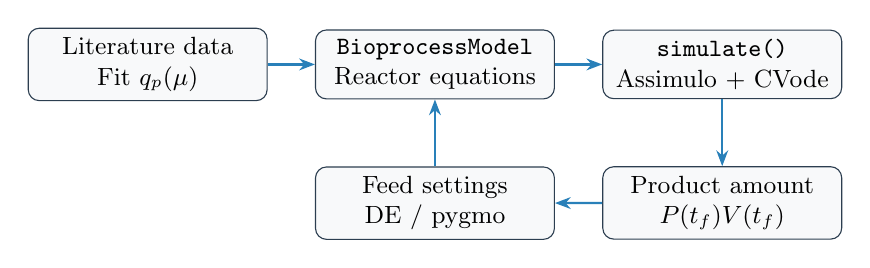
\begin{tikzpicture}[node distance=0.45cm and 0.6cm, every node/.style={align=center},
      flow/.style={rectangle, rounded corners, draw=darkcharcoal, fill=lightbg,
        minimum height=0.85cm, text width=2.8cm, font=\small},
      arr/.style={-{Stealth[length=2mm]}, thick, color=accentblue}]
    \node[flow] (fit) {Literature data\\Fit $q_p(\mu)$};
    \node[flow,right=of fit] (model) {\texttt{BioprocessModel}\\Reactor equations};
    \node[flow,right=of model] (simulate) {\texttt{simulate()}\\Assimulo + CVode};
    \node[flow,below=0.85cm of model] (search) {Feed settings\\DE / pygmo};
    \node[flow,below=0.85cm of simulate] (score) {Product amount\\$P(t_f)V(t_f)$};
    \draw[arr] (fit) -- (model);
    \draw[arr] (model) -- (simulate);
    \draw[arr] (simulate) -- (score);
    \draw[arr] (score) -- (search);
    \draw[arr] (search) -- (model);
  \end{tikzpicture}
  \end{center}
  \vspace{0.2cm}
  \begin{itemize}
    \item Fit $q_p(\mu)$, then vary the feed settings.
    \item Objective: maximise final product $P(t_f)V(t_f)$.
    \item 9 products $\times$ 5 strategies = 45 cases.
  \end{itemize}

\end{frame}

\begin{frame}{Five Feed-Flow Strategies}
  {\small The optimiser chooses the parameters of each feed law.}

  \vspace{0.2cm}
  \begin{center}
  \renewcommand{\arraystretch}{1.2}
  {\footnotesize
  \begin{tabular}{lll}
    \toprule
    \textbf{Strategy} & \textbf{$F(t)$} & \textbf{Free parameters} \\
    \midrule
    Constant & $F_0$ & $F_0$ \\
    Exponential & $F_0 e^{\mu_{set} t}$ & $F_0, \mu_{set}$ \\
    Linear ramp & $F_0 + kt$ & $F_0, k$ \\
    Exponential + linear & $F_0 e^{\mu_{set} t} + kt$ & $F_0, \mu_{set}, k$ \\
    Two-stage & $F_1$ until $t_{switch}$, then $F_2$ & $F_1, F_2, t_{switch}$ \\
    \bottomrule
  \end{tabular}
  }
  \end{center}

  \vspace{0.2cm}
\end{frame}



\begin{frame}{Best Feed Strategy}
  \begin{center}
    \renewcommand{\arraystretch}{1.22}
    {\small
    \begin{tabular}{lll}
      \toprule
      \textbf{Shape} & \textbf{Product} & \textbf{Best strategy found} \\
      \midrule
      Linear & Crl1 Lipase (SCC) & Exponential \\
      Linear & HIP & Exp. + linear / exponential \\
      Linear & Resveratrol & Exponential \\
      Bell-shaped & EPG & Exponential \\
      Bell-shaped & Fab 3H6 & Exponential \\
      Bell-shaped & ROL & Exponential \\
      Hyperbolic & Crl1 Lipase (MCC) & Linear ramp \\
      Hyperbolic & HSA & Linear ramp \\
      Hyperbolic & $\alpha$-Galactosidase & Linear ramp \\
      \bottomrule
    \end{tabular}}
  \end{center}
  \vspace{0.15cm}
  {\small pyFOOMB/CVode results. Exponential and hybrid feeding are nearly tied for HIP.}
\end{frame}

\begin{frame}{Total Product by Feed Strategy}
  \begin{center}
    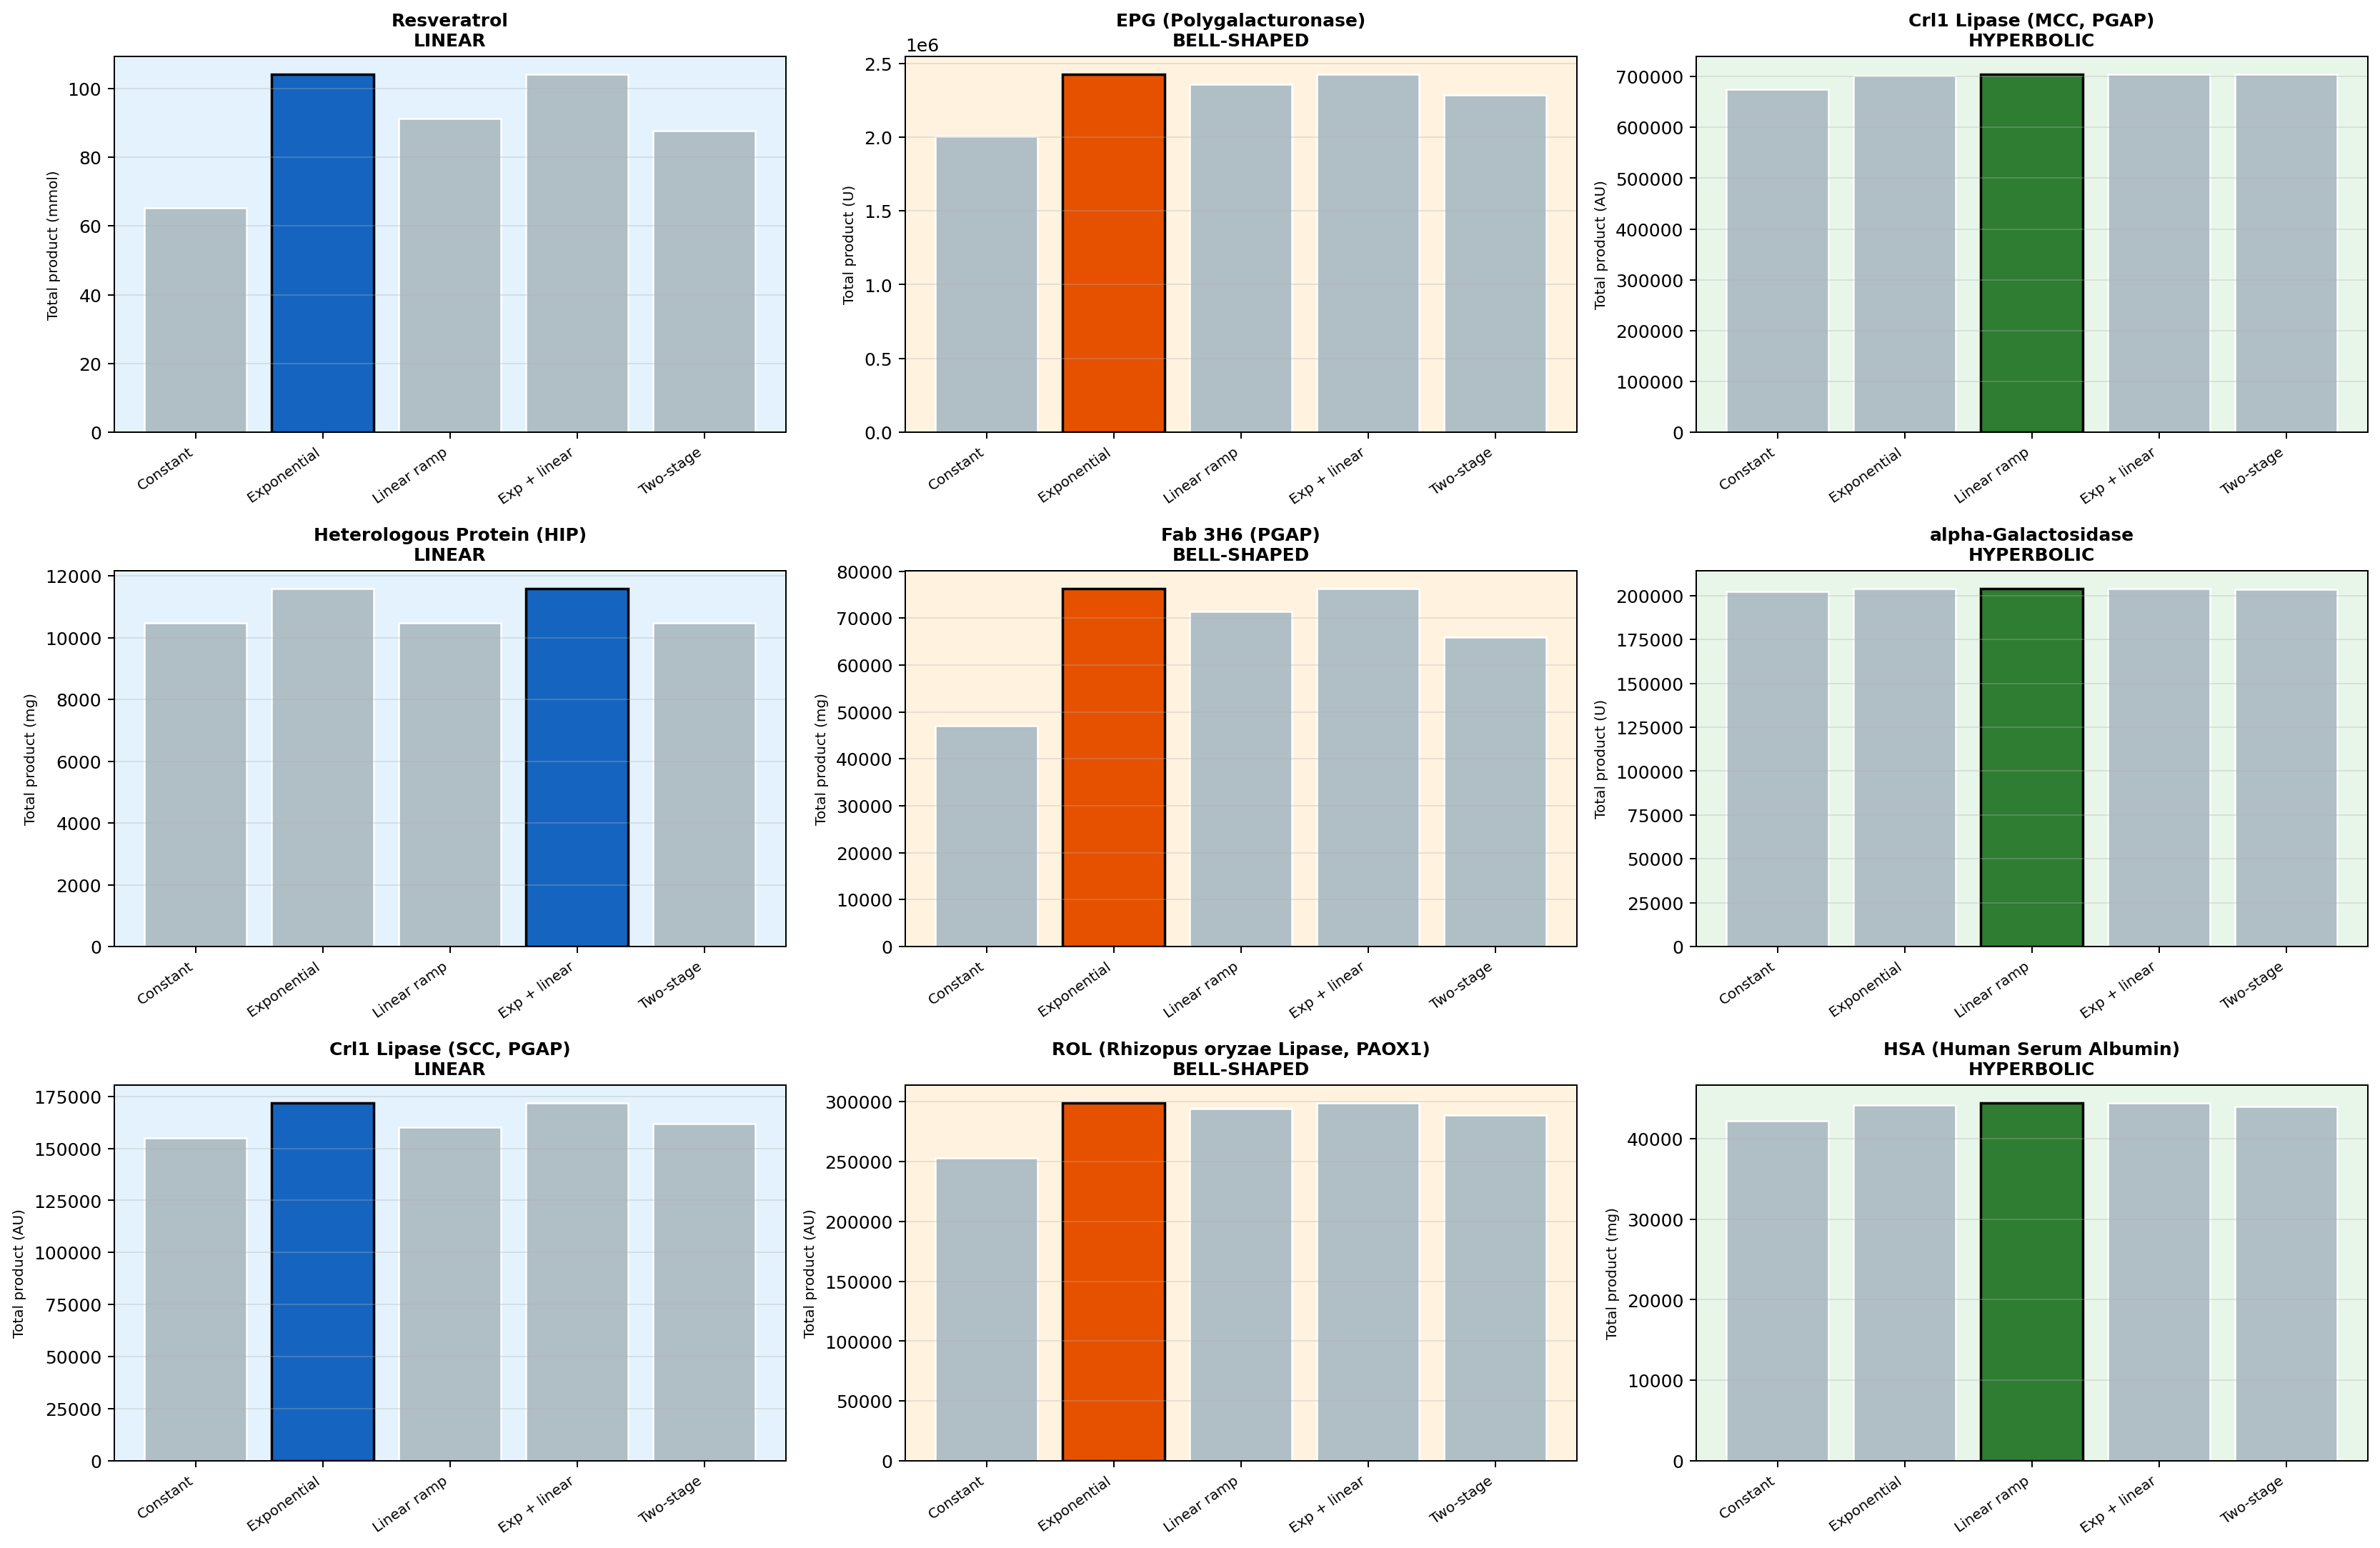
\includegraphics[width=\textwidth,height=0.82\textheight,keepaspectratio]{pyfoomb_results/final/strategy_comparison_five_strategies.png}
  \end{center}
\end{frame}

\begin{frame}{Biomass, Substrate and Product}
  \begin{center}
    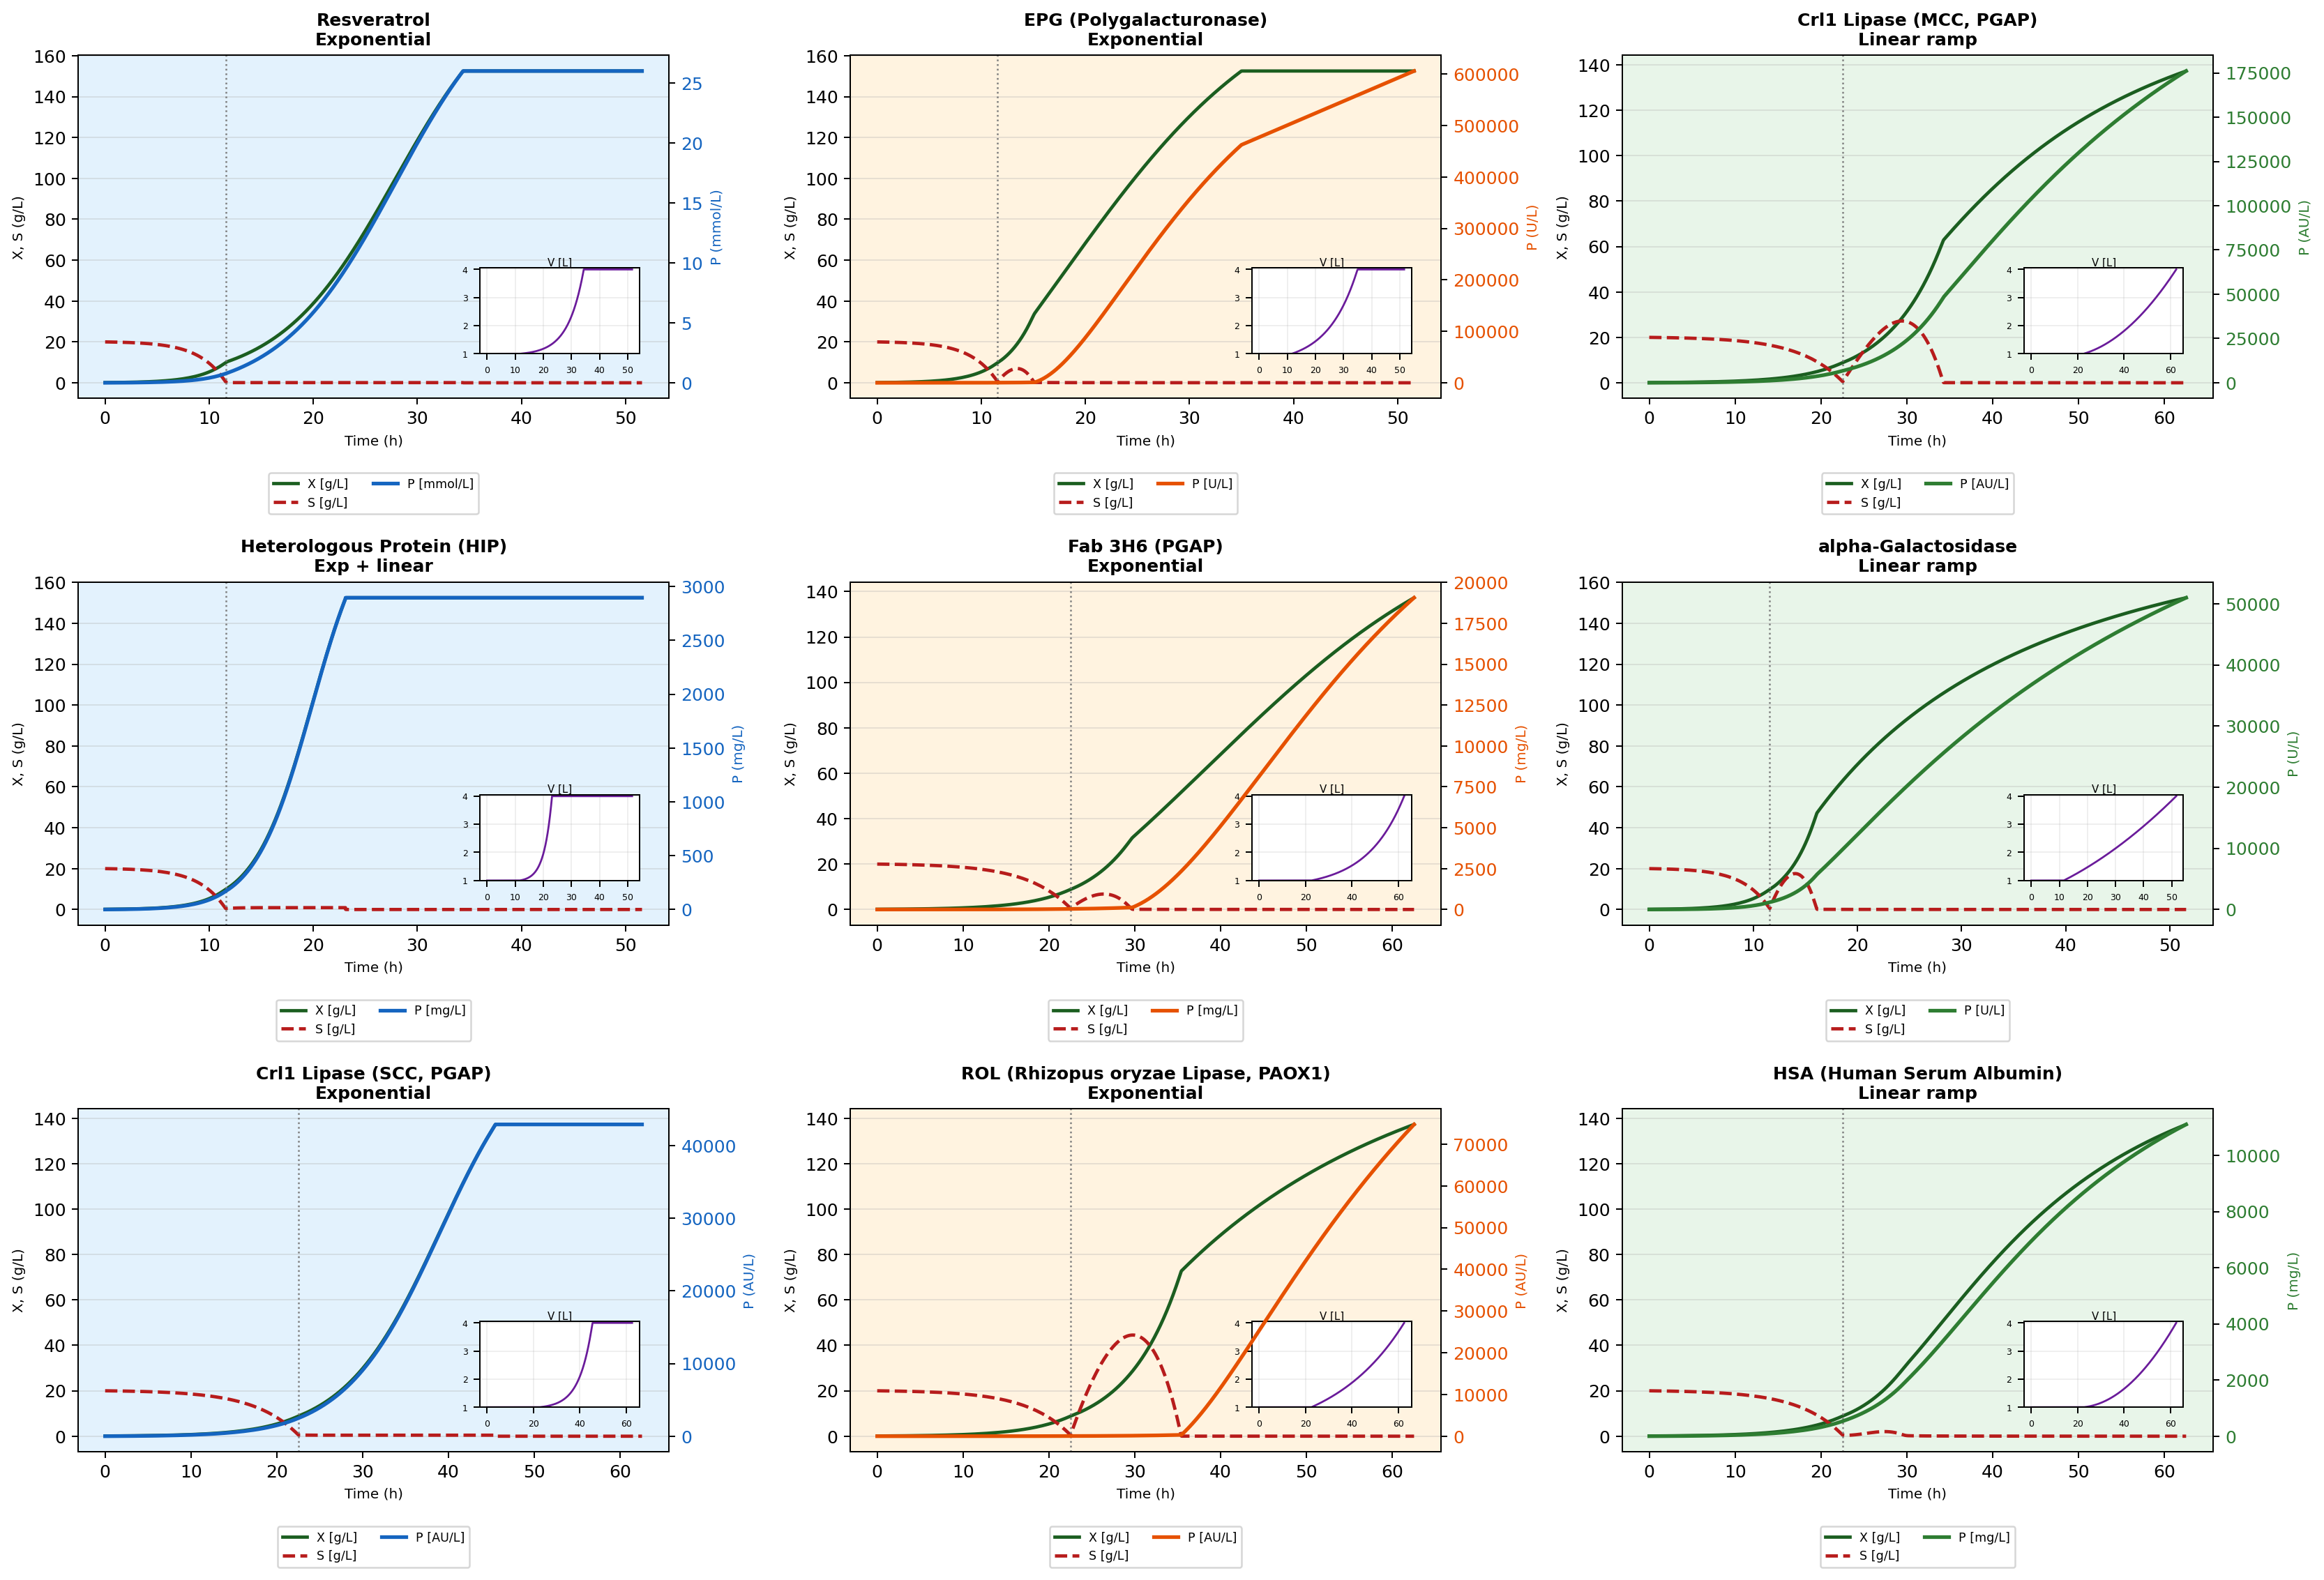
\includegraphics[width=\textwidth,height=0.82\textheight,keepaspectratio]{pyfoomb_results/final/best_profiles_five_strategies.png}
  \end{center}
\end{frame}

\begin{frame}{Findings}
  \begin{center}
    \renewcommand{\arraystretch}{1.35}
    {\small\begin{tabular}{p{2.2cm}p{5.0cm}p{5.0cm}}
      \toprule
      \textbf{$q_p(\mu)$ shape} & \textbf{Best found in the model} & \textbf{Close alternatives} \\
      \midrule
      Linear & Exponential: 2 of 3 products\newline Hybrid: HIP & Exponential and hybrid are within 0.1\% for all three. \\
      Bell-shaped & Exponential: all 3 products & Hybrid is within 0.1\% for EPG, Fab 3H6 and ROL. \\
      Hyperbolic & Linear ramp: all 3 products & Hybrid is close for MCC and HSA; exponential is close for $\alpha$-Gal. \\
      \bottomrule
    \end{tabular}}
  \end{center}
  \vspace{0.1cm}
  \begin{columns}[T]
    \begin{column}{0.48\textwidth}
      \begin{block}{Ranking strength}
        {\small All 9 products have another strategy within 0.1\%.
        A small numerical lead does not establish a practical advantage.}
      \end{block}
    \end{column}
    \begin{column}{0.48\textwidth}
      \begin{block}{Numerical check}
        {\small Same feed settings in CVode and LSODA differ by at most
        0.0052\% in total product across the 45 cases.}
      \end{block}
    \end{column}
  \end{columns}
  \vspace{0.1cm}
  {\small \textbf{Scope:} finite optimisation budgets and shared reactor assumptions.
  Experimental validation is still needed.}
\end{frame}

\begin{frame}{Web Platform: Two Bug Fixes}
  \begin{columns}[T]
    \begin{column}{0.48\textwidth}
      \begin{block}{1. Parallel-request startup crash}
        \begin{itemize}
          \item Worker-pool startup crashed inside a FastAPI request thread.
          \item Initialise the pool at app startup, on the main thread.
        \end{itemize}
      \end{block}
    \end{column}
    \begin{column}{0.48\textwidth}
      \begin{block}{2. Error-alert accessibility}
        \begin{itemize}
          \item Error messages used the ordinary status role.
          \item Use the alert role so screen readers announce errors promptly.
        \end{itemize}
      \end{block}
    \end{column}
  \end{columns}
  \vspace{0.45cm}
  \begin{center}
    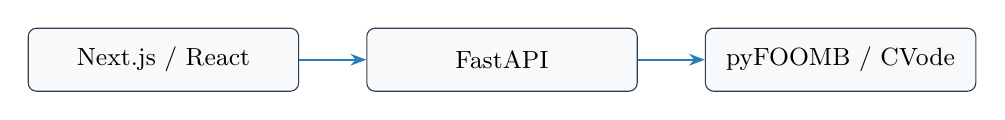
\begin{tikzpicture}[every node/.style={align=center},
      system/.style={rectangle, rounded corners=3pt, draw=darkcharcoal, fill=lightbg,
        minimum height=0.8cm, text width=3.2cm, font=\small},
      arr/.style={-{Stealth[length=2mm]},thick,color=accentblue}]
      \node[system] (a) at (0,0) {Next.js / React};
      \node[system] (b) at (4.3,0) {FastAPI};
      \node[system] (c) at (8.6,0) {pyFOOMB / CVode};
      \draw[arr] (a) -- (b); \draw[arr] (b) -- (c);
    \end{tikzpicture}
  \end{center}
  \vspace{0.15cm}
  {\small \textbf{Next interface task:} add feed-strategy selection and optimisation results.}
\end{frame}



\begin{frame}[plain]
  \vfill
  \begin{center}
    {\LARGE\bfseries\color{darkcharcoal} Thank You}\\[0.3cm]
    {\large\color{accentblue} Questions?}\\[1cm]
    \begin{tabular}{rl}
      \textbf{Student:} & Yashashwi Singhania (23014019) \\
      \textbf{Guide:} & Dr.\ Sharon Mano Pappu J. \\
      \textbf{Lab:} & BPDD, Dept.\ of Biochemical Engineering \\
      \textbf{Institute:} & IIT (BHU) Varanasi \\
    \end{tabular}\\[0.4cm]
    {\small\color{darkcharcoal!60} September 2026}
  \end{center}
  \vfill
\end{frame}

\end{document}
